\documentclass[american,]{article}
\usepackage{lmodern}
\usepackage{amssymb,amsmath}
\usepackage{ifxetex,ifluatex}
\usepackage{fixltx2e} % provides \textsubscript
\ifnum 0\ifxetex 1\fi\ifluatex 1\fi=0 % if pdftex
  \usepackage[T1]{fontenc}
  \usepackage[utf8]{inputenc}
\else % if luatex or xelatex
  \ifxetex
    \usepackage{mathspec}
  \else
    \usepackage{fontspec}
  \fi
  \defaultfontfeatures{Ligatures=TeX,Scale=MatchLowercase}
\fi
% use upquote if available, for straight quotes in verbatim environments
\IfFileExists{upquote.sty}{\usepackage{upquote}}{}
% use microtype if available
\IfFileExists{microtype.sty}{%
\usepackage{microtype}
\UseMicrotypeSet[protrusion]{basicmath} % disable protrusion for tt fonts
}{}
\usepackage[margin=1in]{geometry}
\usepackage{hyperref}
\hypersetup{unicode=true,
            pdftitle={Predicting House Prices with a Linear Regression Model},
            pdfauthor={Kevin Thompson, Sterling Beason, \& Brandon Croom},
            pdfborder={0 0 0},
            breaklinks=true}
\urlstyle{same}  % don't use monospace font for urls
\ifnum 0\ifxetex 1\fi\ifluatex 1\fi=0 % if pdftex
  \usepackage[shorthands=off,main=american]{babel}
\else
  \usepackage{polyglossia}
  \setmainlanguage[variant=american]{english}
\fi
\usepackage{natbib}
\bibliographystyle{apalike}
\usepackage{longtable,booktabs}
\usepackage{graphicx,grffile}
\makeatletter
\def\maxwidth{\ifdim\Gin@nat@width>\linewidth\linewidth\else\Gin@nat@width\fi}
\def\maxheight{\ifdim\Gin@nat@height>\textheight\textheight\else\Gin@nat@height\fi}
\makeatother
% Scale images if necessary, so that they will not overflow the page
% margins by default, and it is still possible to overwrite the defaults
% using explicit options in \includegraphics[width, height, ...]{}
\setkeys{Gin}{width=\maxwidth,height=\maxheight,keepaspectratio}
\IfFileExists{parskip.sty}{%
\usepackage{parskip}
}{% else
\setlength{\parindent}{0pt}
\setlength{\parskip}{6pt plus 2pt minus 1pt}
}
\setlength{\emergencystretch}{3em}  % prevent overfull lines
\providecommand{\tightlist}{%
  \setlength{\itemsep}{0pt}\setlength{\parskip}{0pt}}
\setcounter{secnumdepth}{5}
% Redefines (sub)paragraphs to behave more like sections
\ifx\paragraph\undefined\else
\let\oldparagraph\paragraph
\renewcommand{\paragraph}[1]{\oldparagraph{#1}\mbox{}}
\fi
\ifx\subparagraph\undefined\else
\let\oldsubparagraph\subparagraph
\renewcommand{\subparagraph}[1]{\oldsubparagraph{#1}\mbox{}}
\fi

%%% Use protect on footnotes to avoid problems with footnotes in titles
\let\rmarkdownfootnote\footnote%
\def\footnote{\protect\rmarkdownfootnote}

%%% Change title format to be more compact
\usepackage{titling}

% Create subtitle command for use in maketitle
\providecommand{\subtitle}[1]{
  \posttitle{
    \begin{center}\large#1\end{center}
    }
}

\setlength{\droptitle}{-2em}

  \title{Predicting House Prices with a Linear Regression Model}
    \pretitle{\vspace{\droptitle}\centering\huge}
  \posttitle{\par}
    \author{Kevin Thompson, Sterling Beason, \& Brandon Croom}
    \preauthor{\centering\large\emph}
  \postauthor{\par}
      \predate{\centering\large\emph}
  \postdate{\par}
    \date{Data Science Program, Southern Methodist University, USA \break}

\usepackage{amsmath}
\usepackage[utf8]{inputenc}
\usepackage[T1]{fontenc}
\usepackage{setspace}
\onehalfspacing
\setcitestyle{round}
\newcommand\numberthis{\addtocounter{equation}{1}\tag{\theequation}}

\begin{document}
\maketitle
\begin{abstract}
Price prediction is pivotal for real estate. Homeowners on the sell-side
want to know when to sell, what to renovate, and how much profit they
can expect from their efforts. Homebuyers want to know whether they are
getting a fair price, where to look for homes in their budget, and the
various trade-offs that accompany a purchasing decision. Real estate
companies navigate both sides of real estate; hence, they too are a key
stakeholder. In the first part of our analysis, we estimate the
relationship between house prices, the square footage, and neighborhood
location in Ames, Iowa. In the second part of our analysis, we train a
linear regression model to predict house prices in Ames, Iowa.
\end{abstract}

\section{Introduction}\label{introduction}

Price prediction is pivotal for real estate. Homeowners on the sell-side
want to know when to sell, what to renovate, and how much profit they
can expect from their efforts. Homebuyers want to know whether they are
getting a fair price, where to look for homes in their budget, and the
various trade-offs that accompany a purchasing decision. Real estate
companies navigate both sides of real estate; hence, they too are a key
stakeholder. These stakeholders utilize multiple factors related to real
estate to determine the fair price for the property. These same factors
can be built into a model for price prediction that assists in taking
some of the guess work out of property pricing.

The analysis performed for this paper leverages a data set focused on
the housing market in Ames, Iowa. This data set is from the ``House
Prices: Advanced Regression Techniques'' Kaggle competition
(\citet{Kaggle2016}). In this competition Kaggle competitors attempt
build models that best predict housing prices based on the Ames, Iowa
data set. Over the course of this paper a similar approach to this
specific Kaggle competition will be taken. The first part of the paper
will focus on the Ames, Iowa dataset, provide the reader with detailed
information about the data and any additional variables the team created
for model building. Analysis of this data will then be performed in two
parts. In the first part of our analysis, we estimate the relationship
between house prices, the square footage, and neighborhood location in
Ames, Iowa. In the second part of our analysis, we train a linear
regression model to predict house prices in Ames, Iowa.

The intent of this paper is to provide the reader with an understanding
of how linear regression can be applied to data and the analysis that
must be undertaken to ensure a linear regression model is adequately
developed.

\citet{Sleuth}

\section{Ames, Iowa Data}\label{ames-iowa-data}

The data used for this analysis, described in the sections below, comes
from the Kaggle Competition ``House Prices: Advanced Regression
Techniques'' (\citet{Kaggle2016}). The data set for this competition
contains housing related data for Ames, Iowa. The total data set
contains 2919 observations and 80 features or variables. Although too
numerous to describe here (see the Kaggle website for full descriptors
(\citet{Kaggle2016})), these 80 features relate to quantity and quality
based attributes of a physical property that may interest any of the key
stakeholders (prospective home buyer, home seller, real estate
company/agent). For example the data provides answers to questions such
as: ``How many rooms in the property?'', ``What is the condition of the
kitchen?'', ``What is the location of the property?'', ``Is there a
basement?''. Delving deeper, the data set breaks down into 46
categorical variables and 34 numeric variables.

The categorical variables break down into a relatively equal mix of
nominal and ordinal values (23 nominal and 23 ordinal). The ordinal
variables indicate a grading of various property related components such
as the overall property quality, overall property condition, room
specific quality and room specific conditions. The nominal values
provide information on various conditions of the property such as
building materials used and dwelling type. \citet{DeCock2011}

The numeric variables contain both continuous and discrete values (20
continuous and 14 discrete). The continuous variables indicate
information a prospective stakeholder would like to understand such as
lot size, total square footage, and specific square footage for living
spaces. The discrete variables provide the prospective stakeholder with
an understanding of items such as number of bedrooms, number of
bathrooms, etc. \citet{DeCock2011}

In reviewing the data it was determined that a few variables could be
removed for reasons noted below:

\begin{itemize}
\tightlist
\item
  ID - this field is a record ID field and is not informational for
  analysis
\item
  Pool Quality - this field does not contain enough variation to be
  useful
\item
  Miscellaneous Feature - this field contains minimial information
\end{itemize}

Data quality checks were performed across all remaining variables to
address missing values, inconsistent variable names, and to ensure
consistent ordering of ordinal variables across all variables of the
same type. Comparison analysis was also performed to ensure the variable
ordering was appropriate, as shown in figures X \& X

\section{Analysis Question I}\label{analysis-question-i}

\subsection{Problem Statement}\label{problem-statement}

A local real estate company, Century 21, would like to understand the
relationship between living area of a home and sale prices.
Specifically, the company would like to focus only on sales in certain
neighborhoods (North Ames, Edwards, and Brookside). An estimate (or
estimates) of this information as well as required confidence intervals
should be provided, along with verification of the model assumptions and
addressing of suspicious observations. In the conclusion quantify the
relationship between living area and sale price with respect to these
three neighborhoods.

\subsection{Methodology}\label{methodology}

We begin by fitting the following linear regression model:

\begin{equation}
Price_i = {\beta_0} + {\beta_1}GrLivArea_{i} + {\beta_2}NAmes_{i} + {\beta_3}Edwards_{i} + {\beta_4}GrLivArea_{i}\*NAmes_{i}
+ {\beta_5}GrLivArea_{i}\*Edwards_{i}
+ {\epsilon_i},
\end{equation}

where \(Price_i\) denotes the price of the i-th house, \(NAmes_i\)
denotes whether the i-th observation is located in the North Ames
neighborhood, \(GrLivArea_i\) denotes the above-ground square foot
living area for the i-th house, and \(Edwards_i\) denotes whether the
i-th observation is located in the Edwards neighborhood. The comparison
neighborhood is the Brookside neighborhood. The following two
interaction terms are included to capture the likely difference in the
marginal contribution of living area to sale price between
neighborhoods. \(\epsilon_i\) denotes the error term for the i-th
observation.

We examine a residual plot to verify the assumptions of the OLS
estimator and the hypothesis tests for the coefficients.

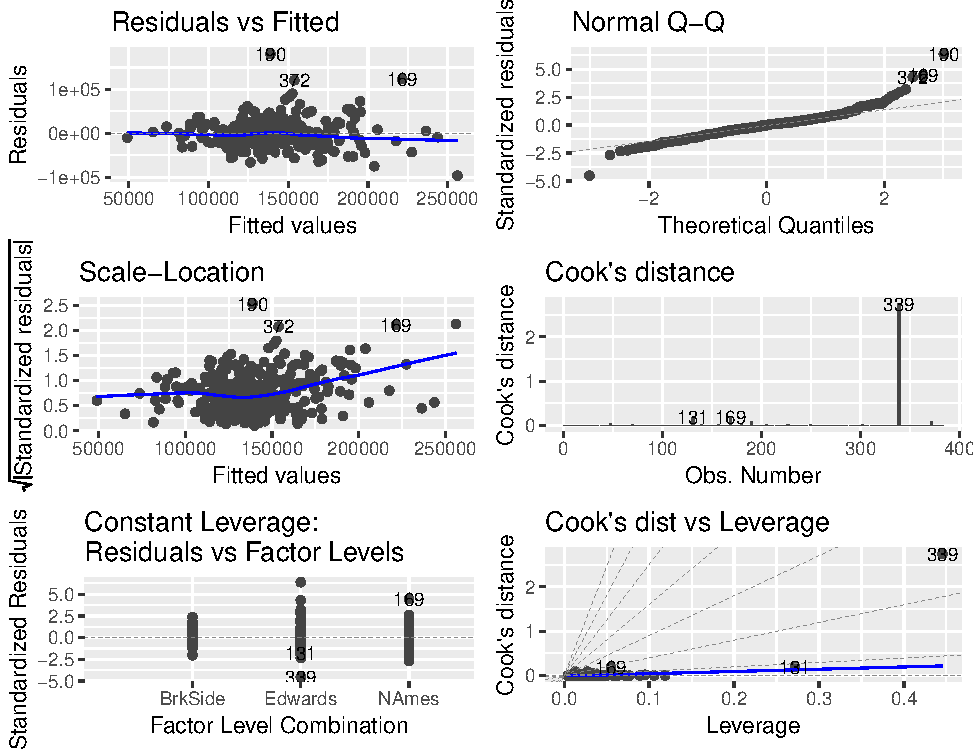
\includegraphics{HousePricesPaper_files/figure-latex/residualplot-1.pdf}

The top-right qq-plot of the studentized residuals suggests moderate
skew and the presence of influential observations. The bottom-right plot
further clarifies the influential observation of interest to be
observation 339, which has significant leverage and distance. Regressing
with and without the observations yields significantly different results
for the Edwards and the Edwards interaction variable, which means we
cannot simply ignore it. We have no reason to believe that significant
measurement error has occurred nor can we find any sufficient reason to
exclude the observation, thus we turn to a log-transformation to reduce
the influence of this observation. We chose the log-transformation in
particular for the sake of interpretability.

Our updated model is:

\begin{equation}
log({Price_i}) = {\beta_0} + {\beta_1}GrLivArea_{i} + {\beta_2}NAmes_{i} + {\beta_3}Edwards_{i} + {\beta_4}GrLivArea_{i}\*NAmes_{i}
+ {\beta_5}GrLivArea_{i}\*Edwards_{i}
+ {\epsilon_i},
\end{equation}

where ``log'' denotes the natural logarithm. We again examine the
residuals to find that the relative influence of observation 339 is
barely lower, though we do get similar results for our question of
interest with and without the observation. Thus, in some sense, the
transformation has weakened the influence of outliers.

We find no evidence of non-constant variance or non-linearity, while the
number of observations gives us sufficient protection from the skewness
of the residuals. We thus conclude that the log-linear model will
suffice for the question of interest.

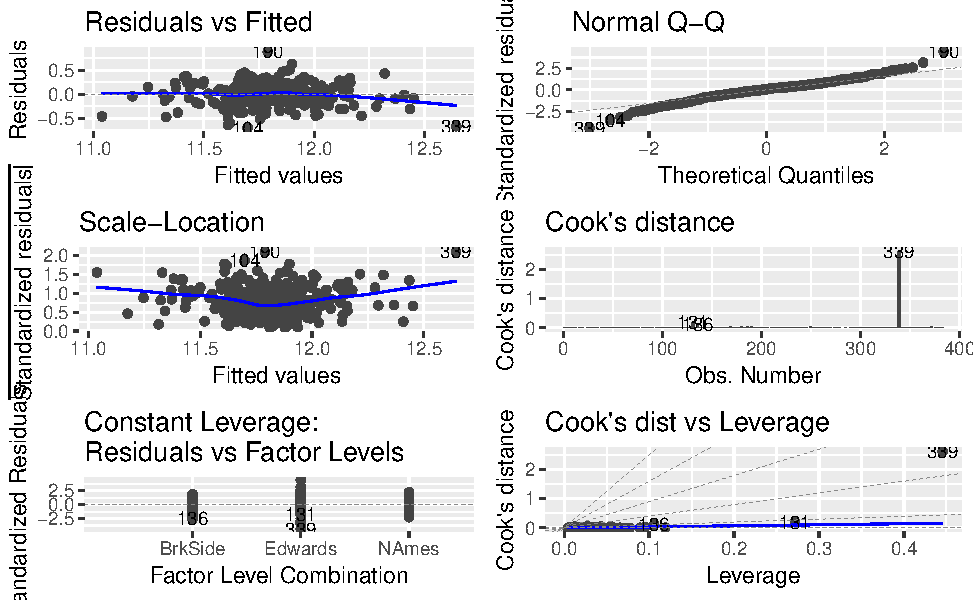
\includegraphics{HousePricesPaper_files/figure-latex/logmodelplot-1.pdf}

\begin{verbatim}
## 
## Call:
## lm(formula = log(SalePrice) ~ GrLivArea + Neighborhood + GrLivArea * 
##     Neighborhood, data = relevantData)
## 
## Residuals:
##     Min      1Q  Median      3Q     Max 
## -0.6963 -0.1044  0.0138  0.1107  0.8862 
## 
## Coefficients:
##                                 Estimate Std. Error t value Pr(>|t|)    
## (Intercept)                    1.079e+01  8.702e-02 124.019  < 2e-16 ***
## GrLivArea                      7.382e-04  6.892e-05  10.712  < 2e-16 ***
## NeighborhoodNAmes              6.517e-01  9.780e-02   6.664 9.48e-11 ***
## NeighborhoodEdwards            6.303e-01  9.842e-02   6.405 4.49e-10 ***
## GrLivArea:NeighborhoodNAmes   -4.141e-04  7.620e-05  -5.435 9.88e-08 ***
## GrLivArea:NeighborhoodEdwards -5.215e-04  7.551e-05  -6.907 2.11e-11 ***
## ---
## Signif. codes:  0 '***' 0.001 '**' 0.01 '*' 0.05 '.' 0.1 ' ' 1
## 
## Residual standard error: 0.2012 on 377 degrees of freedom
## Multiple R-squared:  0.466,  Adjusted R-squared:  0.4589 
## F-statistic: 65.79 on 5 and 377 DF,  p-value: < 2.2e-16
\end{verbatim}

We find a positive, significant association between above-ground living
area square footage and the selling price of a home and that this
significance is maintained between neighborhoods. We estimate that a
one-hundred square foot increase in above-ground living area is
associated with a 7\% increase in the median selling price of a home
with a 95\% confidence interval of {[}6.02\%, 8.73\%{]}. Neither the
estimate nor the significance of this variable changed with the removal
of the observation, even in the base linear model. We also find that the
relationship between square footage and home price changes between
neighborhoods. We estimate the change in median price per additional 100
square-feet in North Ames to be 4\% lower than in Brookside, while the
change in median price per additional 100 square-feet in North Ames is
5\% lower (after back-transforming the coefficients), with 95\%
confidence intervals of {[}-5\%, -2\%{]} and {[}-6\%, -3\%{]},
respectively. That being said, we found that homes in North Ames and
Edwards had larger median home values than Brookside. We estimate the
median home value in North Ames to be 92\% larger (95\% confidence
interval - {[}58\%, 132\%{]}) than Brookside and the median home value
in Edwards to be 88\% (95\% confidence interval - {[}55\%, 128\%{]})
larger than in Brookside. These results cannot be generalized outside of
the sample, nor can we infer a causal relationships from this
observational analysis. Lastly, we must acknowledge that the presence of
outliers, particularly observation 339, may have biased our estimates.
Should we desire to get better estimates of the change in mean/median
price for an additional 100 square-feet of living area, we will need to
either get more data or add additional operational specificity to the
way we define a ``home''.

\subsection{Competing Model
Comparison}\label{competing-model-comparison}

\subsection{Parameters}\label{parameters}

\subsection{Conclusion}\label{conclusion}

\citet{Sleuth}

\citet{Pearl2009}

\citet{Ruppert2015}

\section{Analysis Question II}\label{analysis-question-ii}

\subsection{Problem Statement}\label{problem-statement-1}

Build a predictive model, leveraging techniques learned in DS 6371 only,
to predict sales prices of homes in all of Ames, Iowa. The goal is to
produce four models: a forward selection model, a backward selection
model, a stepwise selection model and a custom model. Each model should
have an adjusted \(R^{2}\), CV Press and Kaggle Score. In the conclusion
describe which model is best at predicting future sale prices of homes
in Ames, Iowa.

\subsection{Assumption Checks}\label{assumption-checks}

\subsection{Competing Model
Comparison}\label{competing-model-comparison-1}

\subsection{Parameters}\label{parameters-1}

\subsection{Conclusion}\label{conclusion-1}

\citet{Hastie2009} \citet{Trefethen1997}

\section{Appendix}\label{appendix}

\renewcommand\refname{References}
\bibliography{HousePrices.bib}


\end{document}
